% !TEX TS-program = Xelatex
% !TEX encoding = UTF-8 Unicode

\documentclass[UTF8]{ctexart}
\usepackage{amsmath}
\usepackage[bottom]{footmisc}
\usepackage{geometry}
\usepackage{hyperref}
\usepackage{graphicx}
\usepackage{figsize}
\usepackage[separate-uncertainty = true,per-mode=symbol]{siunitx}
\usepackage{tabu}
\usepackage{wasysym}
\geometry{left=0.7in,right=0.7in,bottom=0.7in,top=0.7in}

\title{实验十六:霍尔效应测量磁场}
\author{朱寅杰 1600017721}
\date{2017年12月22日}

\begin{document}
\maketitle
\paragraph{测量霍尔电流$I_H$与霍尔电压$U_H$的关系}
励磁电流$I_M=\SI{0.6}{\A}$。分别把电流接霍尔元件的1、2端和3、4端,测$U_H-I_H$的关系。为消除霍尔元件接口的零点误差与各种副效应,将霍尔电流$I_H$与磁场$I_M$分别反向测出四个电压$U_1$(电流与磁场分别取++方向)、$U_2$($+-$方向)、$U_3$($-+$方向)、$U_4$($--$方向),取$U_H=(U_1-U_2-U_3+U_4)/4$,即可消除主要几个副效应的影响。测量的数据见下表:
\begin{center}
\begin{tabu} to \linewidth {X[c]|X[c]X[c]X[c]X[c]|X[c]||X[c]|X[c]X[c]X[c]X[c]|X[c]}
\hline
\multicolumn{6}{c||}{霍尔电流接1、2端}&\multicolumn{6}{c}{霍尔电流接3、4端}\\
\hline
$I_H$/\si{\mA}	&$U_1$/mV	&$U_2$/mV&$U_3$/mV&$U_4$/mV&$U_H$/mV&$I_H$/\si{\mA}	&$U_1$/mV	&$U_2$/mV&$U_3$/mV&$U_4$/mV&$U_H$/mV
\\
\hline
2.001 	&2.67 	&-3.75 	&-3.66 	&3.76 	&3.46 	&9.993 	&-18.72 	&18.35 	&18.67 	&-18.36 	&-18.53 \\
4.001 	&7.35 	&-7.51 	&-7.31 	&7.45 	&7.41 	&8.002 	&-14.97 	&14.70 	&14.96 	&-14.71 	&-14.84 \\
6.002 	&11.06 	&-11.31 	&-11.01 	&11.07 	&11.11 	&5.999 	&-11.23 	&11.02 	&11.23 	&-11.03 	&-11.13 \\
7.997 	&14.69 	&-15.00 	&-14.60 	&14.90 	&14.80 	&4.000 	&-7.49 	&7.34 	&7.48 	&-7.35 	&-7.42 \\
9.999 	&18.45 	&-18.83 	&-18.41 	&18.71 	&18.60 	&2.000 	&-3.75 	&3.67 	&3.74 	&-3.68 	&-3.71 \\
\hline
\end{tabu}
\end{center}
霍尔电流接1、2端时,使用Origin软件拟合得到$U_H=\SI{-.23}{\mV}+\SI{1.88}{\mV/\mA}\times I_H$,相关系数为\num{.99993};霍尔电流接3、4端时候使用软件拟合得到$U_H=\SI{-.003}{\mV}+\SI{1.8536}{\mV/\mA}\times I_H$,相关系数为\num{-1}。可见二者的线性关系十分好。两个斜率在误差范围(经计算,第一个斜率的不确定度在\num{e-2}量级,再考虑电表的允差则两个斜率的不确定度都在这个量级)内是相等的,这符合我们对霍尔元件的预期(无论是接1、2还是接3、4,产生电势差的都是同一个元件厚度$d$)。

\paragraph{测量霍尔元件的灵敏度$K_H$}
保持霍尔电流为$I_H=\SI{9.999}{\mA}$,改变励磁电流$I_M$,用特斯拉计测量磁场$B$,并仿照前面测出霍耳电压$U_H=(U_1-U_2-U_3+U_4)/4$,从而计算出元件的灵敏度$K_H=U_H/ (I_HB)$。所使用的特斯拉计,允差为1\%加两个字。所使用的电压表允差为0.05\%加三个字。测得的数据及其允差列于下表($U_H$由于是中间结果所以多留一位数字):
\begin{center}\begin{tabu} to \linewidth {X[c]|X[c]X[c]|X[c]X[c]X[c]X[c]|X[c]X[c]}
\hline
$I_M$/A	&$B$/mT	&$\delta B$/mT	&$U_1$/mV	&$U_2$/mV&$U_3$/mV&$U_4$/mV&$U_H$/mV  &$\delta U_H$/mV\\
\hline
0.000 	&1.0 	&0.2 &-0.27 	&-0.28 	&0.25 	&0.26 		&0.005		&      0.030 \\
0.100 	&36.1 &	0.6 	&2.73 	&-3.42 	&-2.75 	&3.39 		&3.073		&	   0.038   \\
0.200 	&72.2 &	0.9 	&5.80 	&-6.48 	&-5.83 	&6.45 		&6.140		&0.045         \\
0.300 	&107.8&	1.3  	&8.86 	&-9.52 	&-8.87 	&9.49			&9.185	&0.053           \\
0.400 	&143.9&	1.6  	&11.99 	&-12.71 	&-12.06 	&12.67 	&12.358	&0.061 	\\
0.500 	&180.5&	2.0  	&15.05 	&-15.76 	&-15.12 	&15.71 	&15.410	&0.069 	\\
0.600 	&216.2&	2.4  	&18.18 	&-18.89 	&-18.17 	&18.74 	&18.495	&0.076 	\\
0.700 	&252.8&	2.7  	&21.39 	&-21.96 	&-21.33 	&21.90 	&21.645	&0.084 	\\
0.800 	&289.7&	3.1  	&24.31 	&-25.00 	&-24.45 	&24.99 	&24.688	&0.092 	\\
0.900 	&323.4&	3.4  	&27.26 	&-27.42 	&-27.44 	&28.03 	&27.538	&0.099 	\\
1.000 	&361.2&	3.8  	&30.40 	&-30.87 	&-30.26 	&30.77 	&30.575	&0.106 		\\
\hline
\end{tabu}\end{center}
要计算出$K_H$的值,也就要拟合出$U_H-B$直线的斜率。然而现在$U_H$与$B$都带有着\num{e-2}左右不确定度(由允差折算得到),因此我们使用York法\footnote{York, D. (1968). Least squares fitting of a straight line with correlated errors. \emph{Earth and planetary science letters}, 5, 320-324.}进行线性拟合,它可以给各个带有不确定度的数据点在最小二乘时分配一个合理的权重,并可以计算各拟合量的不确定度。\footnote{具体的算法见\url{https://www.originlab.com/doc/Origin-Help/Ref-Linear-XErr\#Quantities_.28York_Method.29}}操作中我们可以使用Origin软件一步完成所有的拟合计算操作,毋须多费人工笔墨。由该算法算出的结果为
\[U_H=\SI{-.062(18)}{\mV}+\SI{.08568(22)}{\V/T}\times B\]
其Pearson相关系数为\num{.99997},归一化卡方$\chi_\nu^2=\num{.73285}$。电流表的允差为0.5\%加四个字,得霍尔电流$I_H=\SI{10.00(3)}{\mA}$,故$K_H=\SI{.08568(22)}{\V/T}\div I_H=\SI{.08568(22)}{\V/T}\div\SI{10.00(3)} {\mA}=\SI{8.57(3)}{\ohm/T}$。

用以上算出的$K_H$,反推出各$I_M$对应的磁场:
\begin{center}\begin{tabu}to\linewidth{X[c]|X[c]X[c]X[c]X[c]X[c]X[c]X[c]X[c]X[c]X[c]X[c]}
  \hline
$I_M$/A	&0.000 &0.100 &0.200 &0.300 &0.400 &0.500 &0.600 &0.700 &0.800 &0.900 &1.000\\
\hline
$B_\ominus$/mT	&0.058 &35.9 &71.6 &107.2 &144.2 &180 &216 &253 &288 &321 &357\\
  \hline
\end{tabu}\end{center}
作出磁化曲线见附页。
\paragraph{测量电磁铁磁场沿水平方向分布}
取励磁电流为$I_M=\SI{0.6}{\A}$,霍尔电流为$I_H=\SI{10.000}{\mA}$,测量霍尔元件在$x$方向上不同位置(坐标从游标上读出)的霍耳电压,用上面算得的$K_H$折算成磁感应强度。考虑到副效应带来的零点问题,因此我们测量了关闭磁场时霍尔电压为$U_1^{\ominus}=\SI{-.29}{\mV}$,则磁场可由$B=(U_1-U_1^{\ominus})/(I_HK_H)$算出。所得到的数据见下表。由此作出磁场分布曲线见附页。
\begin{center}\begin{tabu}to\linewidth{X[c]|X[c]X[c]X[c]X[c]X[c]X[c]X[c]X[c]X[c]X[c]X[c]}
  \hline
$x$/mm	&41.0 &50.3 &65.0 &69.3 &71.3 &72.3 &73.5 &74.6 &75.8 &76.9\\
\hline
$U_1/mV$	&18.26 &18.28 &18.25 &18.00 &17.02 &15.55 &13.40 &11.16 &9.13 &7.30\\
$B_\ominus$/mT	&216.5 &216.7 &216.4 &213.5 &202.0 &184.9 &159.8 &133.6 &109.9 &88.6 \\
  \hline\hline
$x$/mm&78.0 &79.1 &80.5 &82.3 &85.0 &88.7 &92.8 &95.0 &100.0 &$(\infty)$\\
\hline
$U_1$/mV	&6.06 &5.03 &4.18 &3.37 &2.57 &1.93 &1.49 &1.30 &0.95	&-0.29 \\
$B_\ominus$/mT	&74.1 &62.1 &52.2 &42.7 &33.4 &25.9 &20.8 &18.6 &14.5 &(0.0)\\
\hline
\end{tabu}\end{center}
\paragraph{分析讨论}
在测磁化曲线时,本可以直接用特斯拉计的读数。但由于用霍尔元件的拟合直线计算出的磁场大小的不确定度较小(斜率$U_H/B$的相对不确定度只有0.26\%,合成入电压表允差(按0.5\%计),总的不确定度也只有千分之四。而特斯拉计的允差可达百分之一以上,折成不确定度是比间接算法高很多的),所以还是使用间接计算结果来画磁化曲线的图。

电磁铁的磁化曲线基本呈线性,这符合我们对普通电磁铁的认识($B=\mu_0nI$)。从磁场分布看,靠近中间的地方磁场基本保持均匀,而出了这一范围磁场开始迅速减小,也和我们对通电螺线管式的磁场(这里无非是加了一个铁芯的通电螺线管)的认识相符。

在$I_M=0$时依然能测出非零的$U_H$电压,并且可以看到反向$I_H$时$U_H$随之反向。这一效应主要是1、2两个接口并非完全处于电流场的等势面上,导致通电流以后测电压会有一个先天的零点偏差造成的。
\begin{figure}
\centering
\SetFigLayout{2}{2}
\subfigure[霍尔电流接1、2端时的$U_H-I_H$直线拟合线。十分抱歉采数据的时候没有采$I_H=0$处的数据,所以图线没有画到原点,最后来不及重画了,请老师手下留情。]{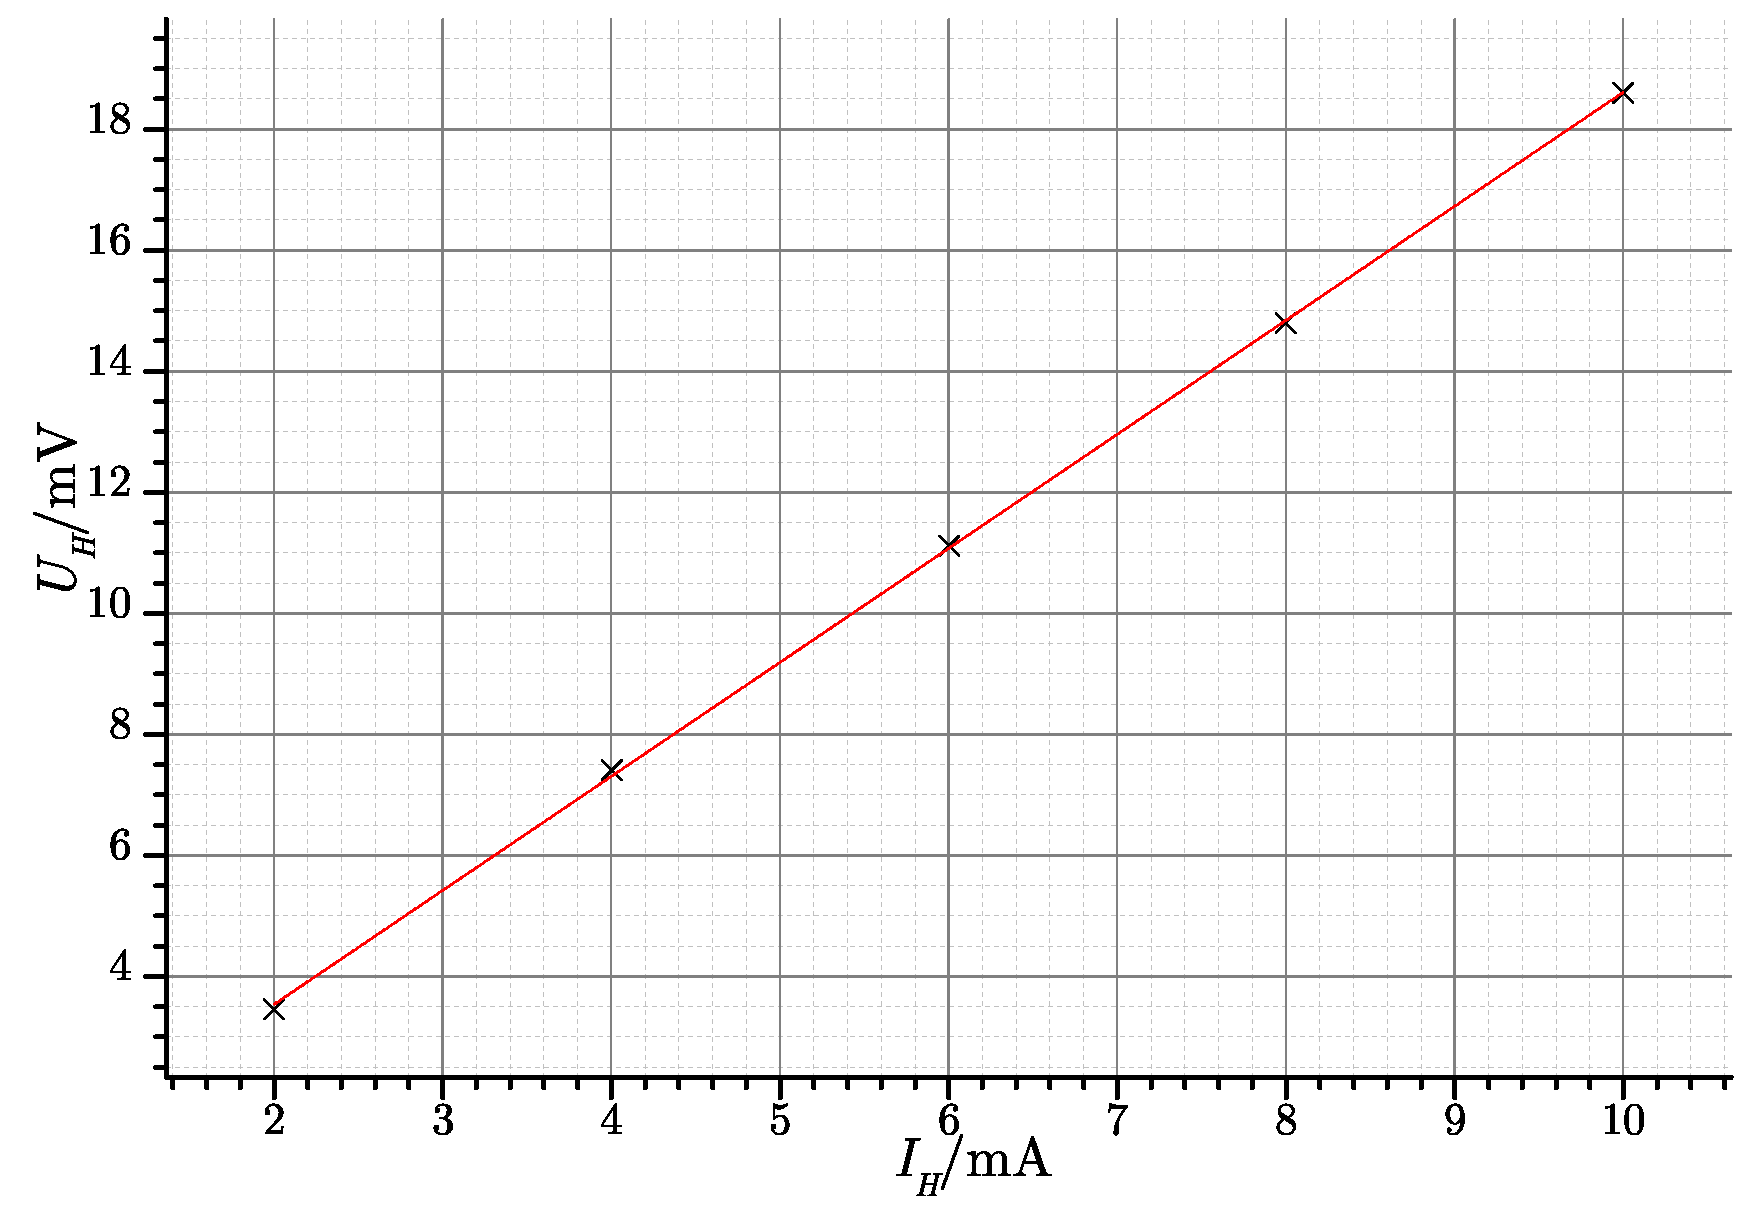
\includegraphics[width=0.49\linewidth]{UI+.eps}} \hfill
\subfigure[霍尔电流接3、4端时的$U_H-I_H$直线拟合线。十分抱歉采数据的时候没有采$I_H=0$处的数据,所以图线没有画到原点,最后来不及重画了,请老师手下留情。]{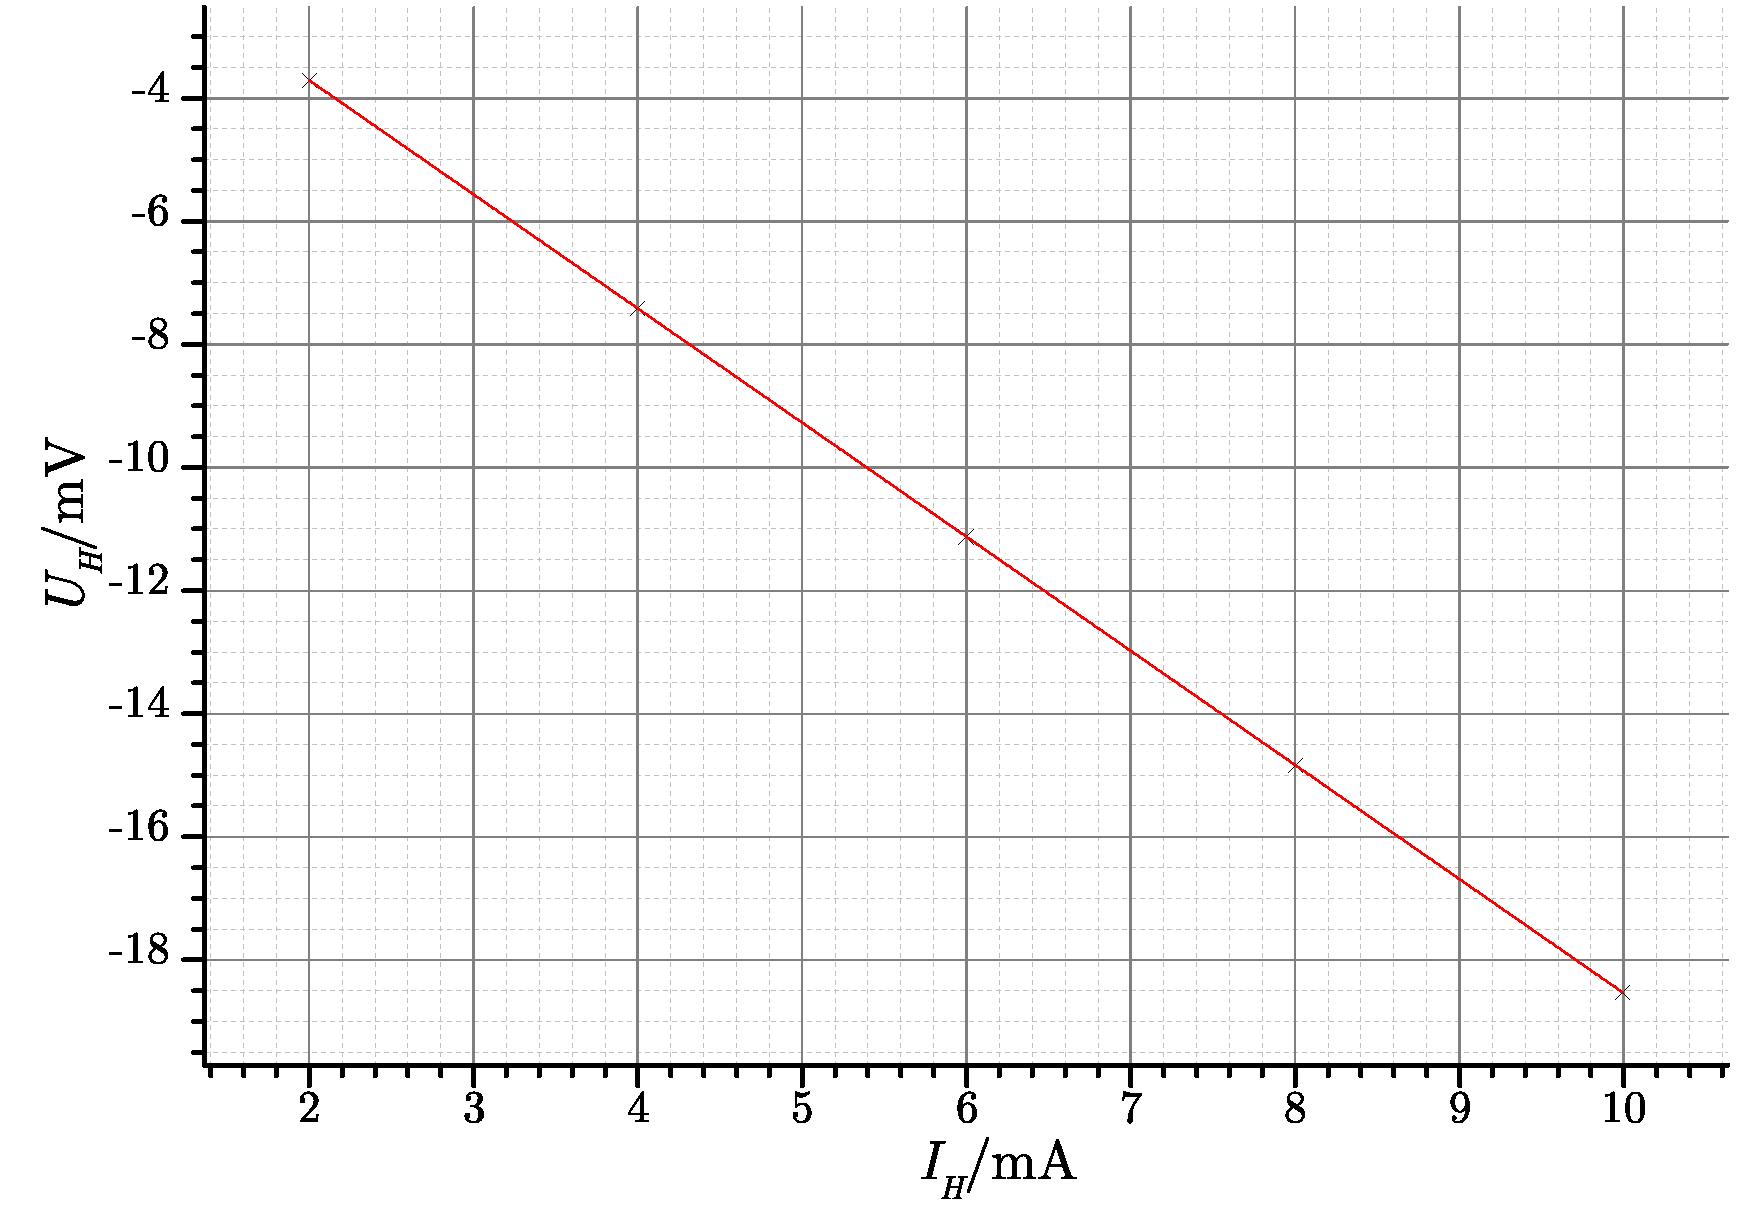
\includegraphics[width=0.49\linewidth]{UI-.eps}} \\
\subfigure[$B-I_M$的磁化曲线。]{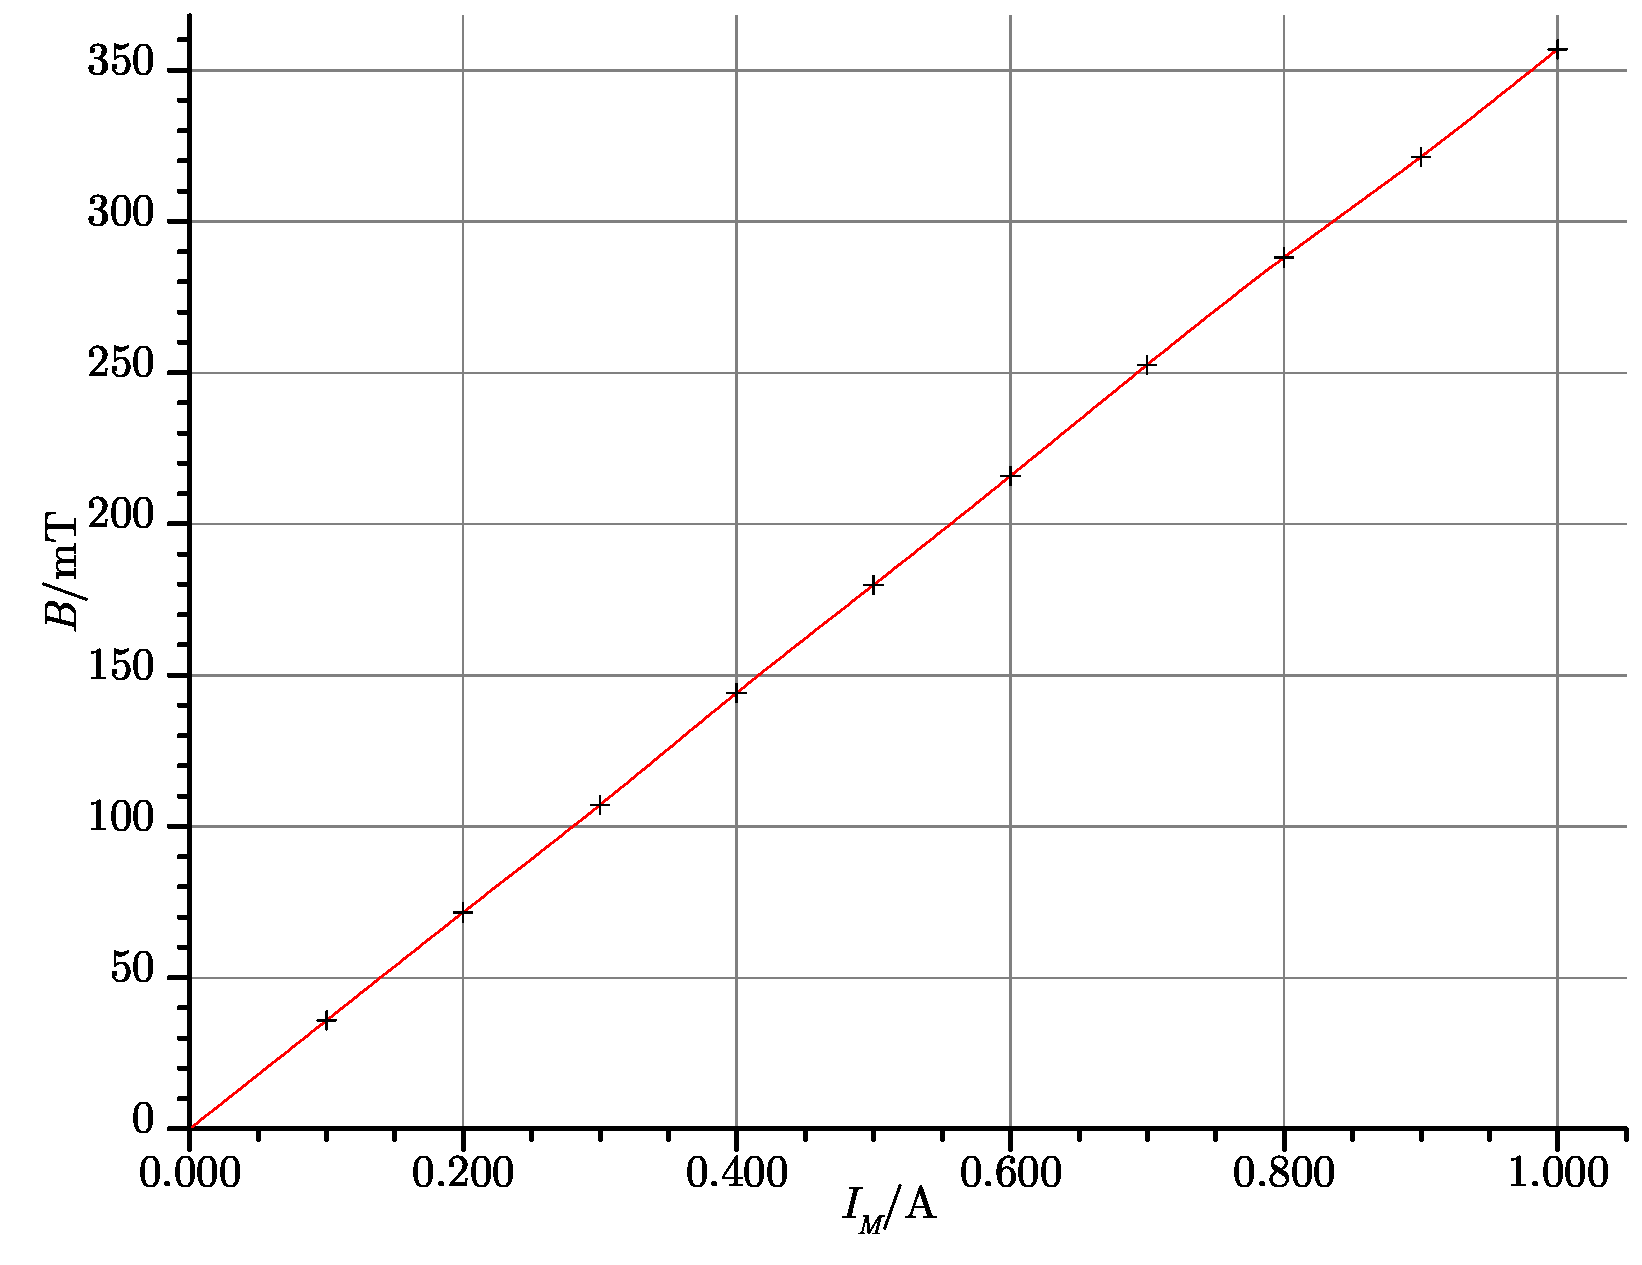
\includegraphics[width=0.49\linewidth]{BI.eps}} \hfill
\subfigure[磁场$B$在水平方向$x$上的分布曲线。]{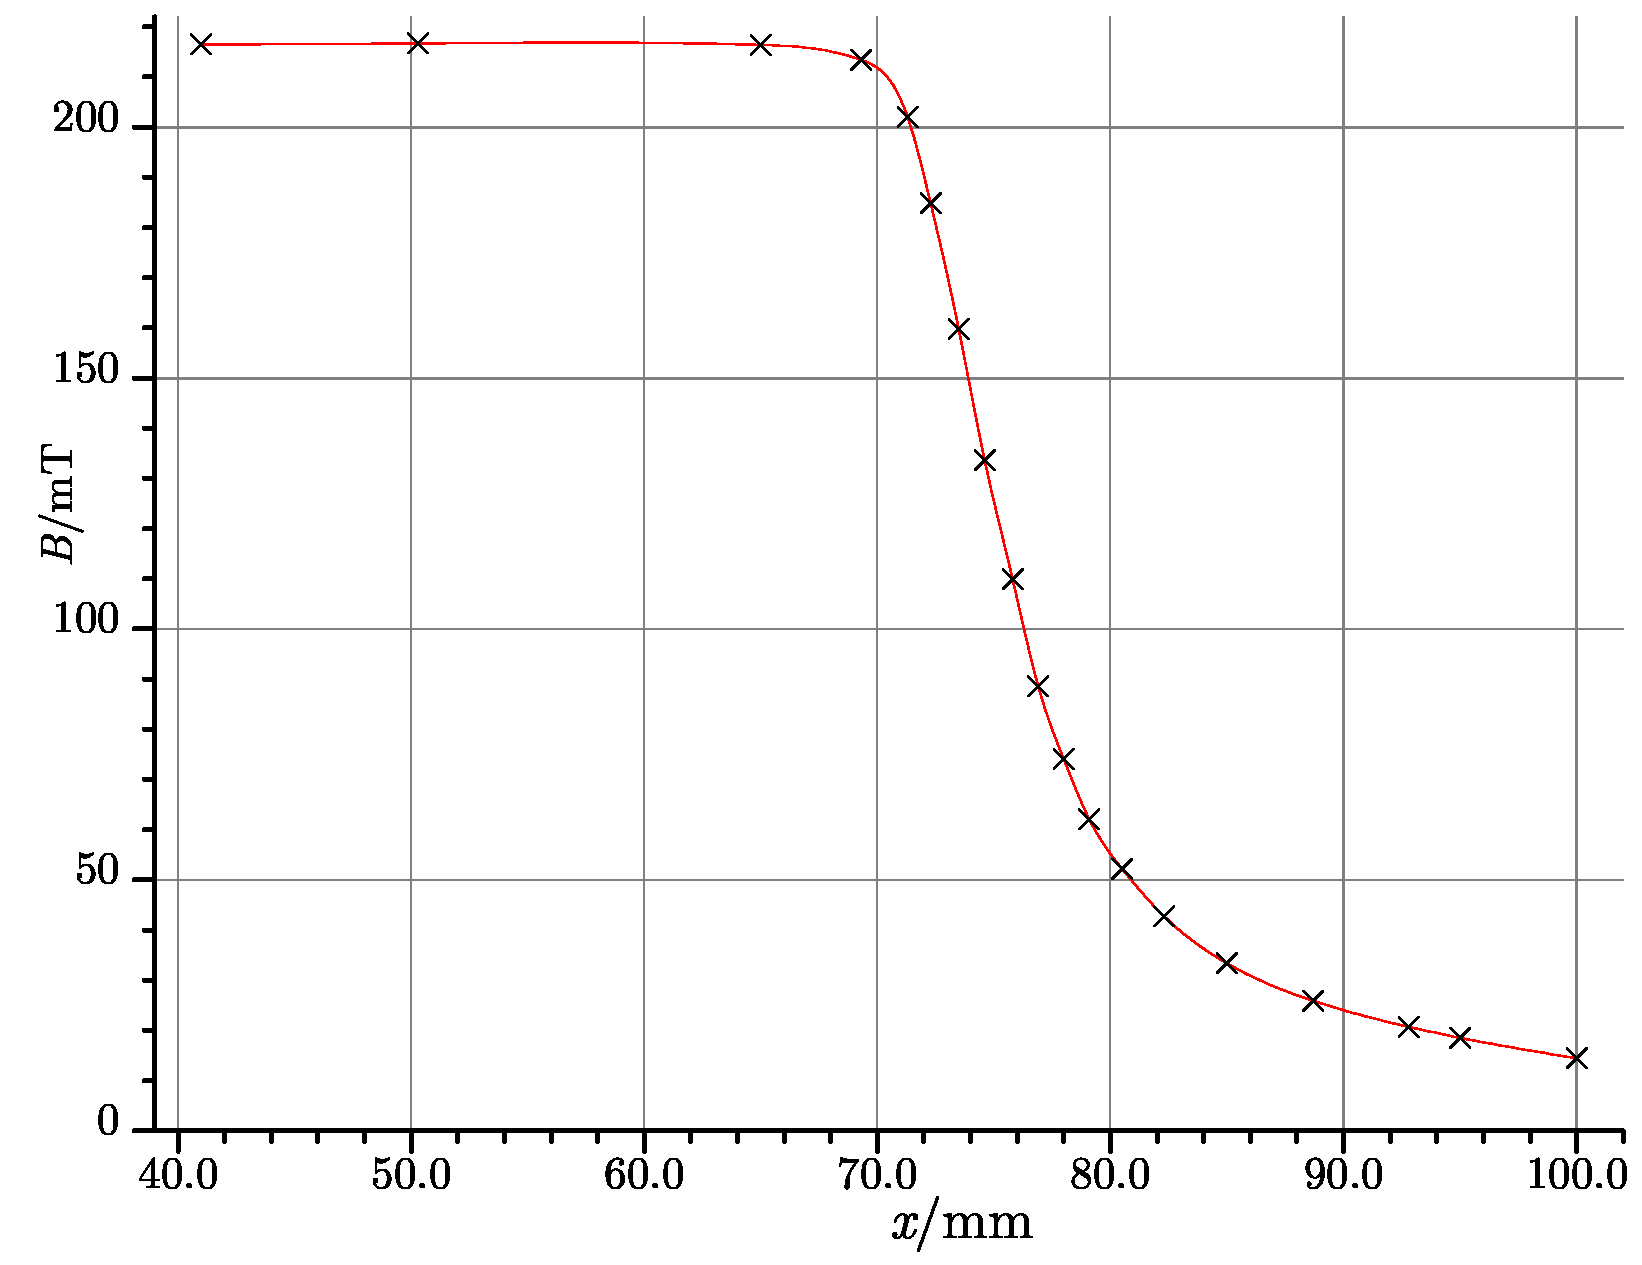
\includegraphics[width=0.49\linewidth]{Bx.eps}} \\
\end{figure}
\end{document} 